% LaTeX-chinese-template v0.4
% https://github.com/CTeX-org/ctex-kit/
%
% You may need to check the instructions at the end of this file.
% See the manual for the collection CTeX for more details.
%
%\documentclass[UTF8,zihao=-4,a4paper,fancyhdr,fntef]{ctexrep}
\documentclass[UTF8,12pt,a4paper,fancyhdr,fntef]{report}
\usepackage{fancyhdr}
\usepackage[top=3cm, bottom=2.5cm, left=2.5cm, right=2.5cm, head=0.5cm, headsep=0.5cm, foot=0.5cm]{geometry}
%\CTEXsetup[number={\arabic{chapter}}, beforeskip={0pt}]{chapter} %format={\zihao{-3}\centering
%\CTEXoptions[contentsname={目\quad 录}]

% Alan: begin the font trial
% Euler for math | Palatino for rm | Helvetica for ss | Courier for tt
\renewcommand{\rmdefault}{ppl} % rm
%\linespread{1.05}        % Palatino needs more leading
\usepackage[scaled]{helvet} % ss
\usepackage{courier} % tt
%\usepackage{euler} % math
\usepackage{eulervm} % a better implementation of the euler package (not in gwTeX)
\normalfont
\usepackage[T1]{fontenc}
% Alan: end the font trial

\newcommand\specialchapter[1]{
    \chapter*{#1}\addcontentsline{toc}{chapter}{#1}
    \markboth{#1}{}\phantomsection}

%\renewcommand{\headrulewidth}{0.5pt}
\pagestyle{fancy}
\fancyhead[l]{{
\includegraphics[scale=.025]{PearLogo.eps}~}\fancyplain{}{\sl\rightmark}}
%\lhead{\zihao{5}
\includegraphics[scale=.025]{PearLogo.eps}~白皮书}
%\fancyhead[r]{\zihao{5}\fancyplain{}{\sl\leftmark}}
%%\fancyhead[H]{\zihao{5}}
%\fancyfoot[c]{\zihao{-5}\rm\thepage}

\newcommand*{\keywords}[1]{\noindent\textbf{Keywords: }#1}
\newcommand*{\cnkeywords}[1]{\noindent\textbf{关键词: }#1}

\title{
\includegraphics[scale=.25]{PearLogo.eps} \\The PRCToken White Paper}
\author{JIANG, Yinghao\\
	\href{mailto:j@pear.hk}{\nolinkurl{(j@pear.hk)}}
}

\usepackage{mathpazo,amsmath,amsfonts,amssymb,epsfig,enumerate,bbm,calc,color,ifthen,capt-of} % original was times, but I think it's ugly; we use the same as IEEE CompSoc
\usepackage{algorithm,algpseudocode}
\usepackage{hyperref}
\PassOptionsToPackage{hyphens}{url}
%\usepackage{breakurl}
\usepackage{geometry}
\usepackage{array}
\usepackage{forest}
\usepackage[absolute,overlay]{textpos}
\usepackage{color,graphicx}
\usepackage{multirow}
\usepackage{booktabs,threeparttable}
\usepackage[formats]{listings}

\usepackage[font=small,justification=centering]{caption}
%\usepackage[font=footnotesize]{subcaption}

\def\UrlBigBreaks{\do\/\do\-\do:\do\_\do\#\do\?}

\usepackage{makecell}
\usepackage{tabularx}


\usepackage{pgfplots,pgfplotstable}
\usepackage{sfmath}
\usepackage{xcolor}

\usepackage{listings}

\usepackage{tablefootnote}

\renewcommand{\vec}[1]{\mathbf{#1}}

\usepackage{tikz}
\usetikzlibrary{arrows,shapes,positioning,shadows,trees,fit,calc}
\tikzset{font=\footnotesize}
\tikzset{
  basic/.style  = {draw, rectangle},
  root/.style   = {basic, rounded corners=2pt, thin, align=center,
                   fill=green!30},
  level 2/.style = {basic, rounded corners=6pt, thin,align=center, fill=green!60},
  level 3/.style = {basic, thin, align=left, fill=pink!60}
}

\tikzset{font=\footnotesize}

\hypersetup{
	pdftitle={The PRCToken White Paper},    % title
	pdfauthor={JIANG, Yinghao},     % author
	pdfsubject={White Paper of the Pear Coin Token (PRCToken)},   % subject of the document
	pdfkeywords={Fog Computing, Crowdsourcing, Shared Computing, CDN, Blockchain, Token}, % list of keywords
}

\begin{document}
\maketitle
\pagenumbering{roman}


\specialchapter{Abstract}
% This version may be obsolete, please download the latest from: \url{https://pear.hk/thesis.pdf}\\
With the rapid growth of connected Internet of Things (IoT) devices and online media traffic demand, as well as the increasingly conspicuous limitations of the Cloud, the Fog has emerged to be a promising research topic that is breeding another transformation in computing. Pear is a start-up implementing fog computing technology from concept into reality. Conforming to the ``XaaS'' philosophy, incorporating the crowdsourcing paradigm, and agglomerating the Sharing Economy, Pear is able to scale up a network with a pool of resources, provide reliable services and make a subset of fog touch the ground. 

In this white paper, we provide a retrospective view of development in related fields over the past two decades, with highlights on the lessons learned. We abstract them to metaphors and analogies that indicate and inspire our philosophy, choices and decisions. We generalise the working fashion to a unified model, and we give solutions to key problems. We also introduce several of Pear's on-going business projects from both technological and business perspectives. Algorithmic, protocolic and architectural design principles are also discussed, along with a business plan.   

%\vspace{12pt}
%\keywords{Fog Computing, Crowdsourcing, Shared Computing, CDN, Blockchain, Token}


%\specialchapter{Abstract}

%This document was typesetted and compiled with the ~\LaTeX~ template by my own. Anyone senior who is interested

%in writing technical/academic reports with it can acquire a copy from me at any time (though there may exist some boring bugs).


%\vspace{12pt}

%\keywords{CDN, NFS, Back to Source, Elimination, Deletion, Directory Traversal, Parallelism, Power-law Distribution}

\tableofcontents
\newpage
\pagenumbering{arabic}

\chapter{Introduction}\label{sec-introduction}
Before there were mobile devices, there was media content. But now that there are mobile devices, 
there is even more media content, and both media content consumption and generation lie at the heart of mobile applications. 

For thousands of years, people have never exhausted their desire to feast their eyes on something visually and ``illusionally'' attractive (see Figure~\ref{fig:visual-feasts}). 
Since photography and television devices were invented, people have begun to spend more and more time on virtual scenes in front of their eyes, be it a photograph, a movie screen, a TV screen, a PC monitor, a tablet PC, a smartphone, or a VR\footnote{Virtual Reality. Example phenomenal device: Oculus of Facebook.} headset.  
Small wonder that VR and AR\footnote{Augmented Reality. Example killer app: Pokemon Go by Niantic.} are subsequently and concurrently two of the hottest topics in consumer electronics today. 
\begin{figure}[ht]
	\centering
	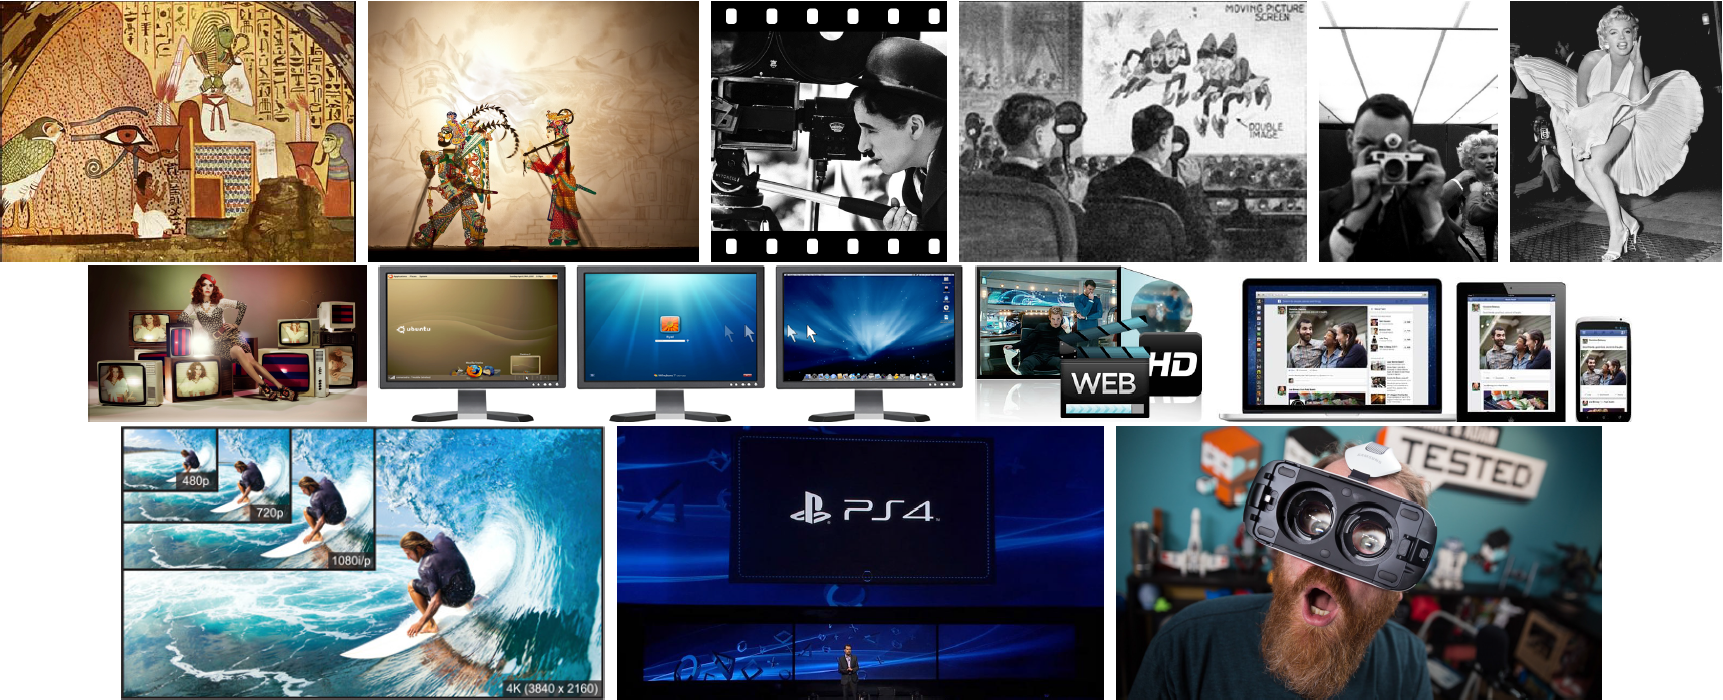
\includegraphics[width=\linewidth]{fig/general/visual-feasts.png}
	\caption{Human's visual feasts in history.}\label{fig:visual-feasts}
\end{figure}

Billions of people now enjoy huge screens and high definition videos. For entertainment,  people are now greedily expecting to experience as many details in the virtual world as in reality. 
This is why nowadays we have 720p, 1080p, 2K, and 4K resolution pictures and videos, with 8K to 16K coming in the near future. 
Moreover, since VR technology tends to be prevalent in gaming and entertainment, billions of mobile devices are ready to fetch these super high definition VR videos from the Internet to please their masters. 
For Internet television, the elementary-level resolution is 1080p and the standard-level is 4K; in VR/AR, 4K is considered basic, while it is expected that the standard-level will soon become 16K. 

What kind of network throughput problems will we face with the rise and rapid use of VR/AR devices? Figure~\ref{fig:bitrate-resolution} roughly illustrates the relationship between the resolutions and the bitrates required with the H.265 (HEVC) coding standard. 

\begin{figure}[ht]
	\centering
	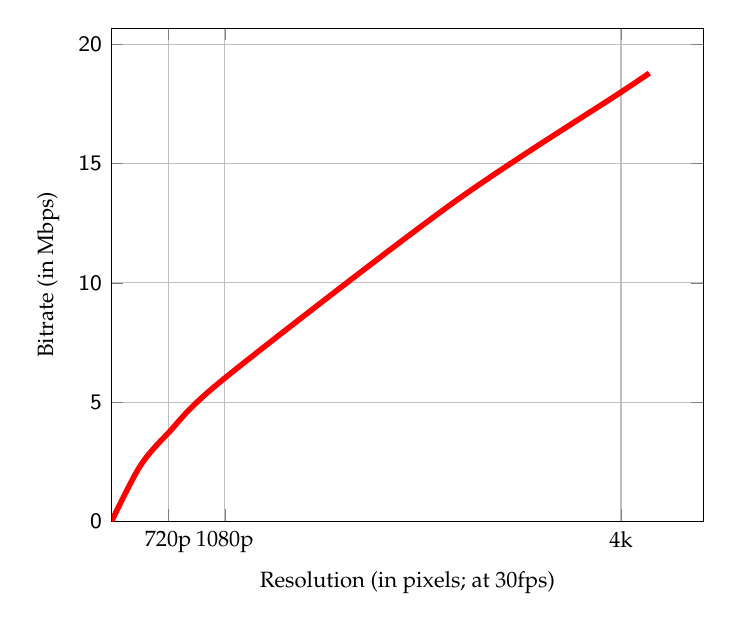
\begin{tikzpicture} %[>=latex]
\begin{axis}[
width=0.75\textwidth,
%line width=2,
%symbolic x coords={2012, 2013, 2014, 2015, 2016},
xtick={2,4,18},
xticklabels={720p,1080p,4k},
%minor xtick={0,1,...,18},
grid=both,
ymin=0,
xmin=0,
xlabel=Resolution (in pixels; at 30fps),
ylabel=Bitrate (in Mbps),
%enlarge x limits=0.1,
%xticklabel style={text width=0.2\textwidth,align=flush left},
]
\addplot[line width=2pt,smooth,color=red] coordinates {
	(0,0)
	(1,2.300)
	(2,3.700)
	%(3,5050)
	(4,6.006)
	(12,13.300)
	(18,18.000)
	(19,18.800)
};
%\draw[red] plot [smooth] coordinates {(0 0) (2,3700) (4,6006) (18,18000)};
\end{axis}
\end{tikzpicture}
	\caption{Bandwidth required for delivering various videos.}\label{fig:bitrate-resolution}
\end{figure}

To put this in perspective, let's look at the coming explosion in demand for network throughput. With the rapid progress of low-power wireless communications and the evolution of micro-sensors, the not-really-new concept of IoT begins to touch ground in novel fields like smart wearables, smart agriculture, smart homes, smart buildings, smart environments, smart cities, smart transportation, smart enterprises and smart hospitality. It is an undoubted trend that there will be an exponentially growing number of devices connecting to the Internet. 
In 2011, Cisco predicted that there would be 25 billion devices connected to the Internet by 2015 and 50 billion by 2020 \cite{evans2011internet}. 

Just imagine if these devices continually send 1K total-sized \texttt{HeartBeat} messages to the cloud in 1-second intervals. 
What kind of pressure will this put on backbone networks and cloud services in general? What challenges will network engineers face in coming years? And what new solutions will emerge? 

These challenges have forced the emergence of fog computing, a fairly new paradigm which basically moves some elements of Cloud Computing closer to the end users, especially in a machine-to-machine (M2M), collaborative platform; these elements include compute, storage, and networking devices \cite{Bonomi:2012:Fog:IoT}. 

Pear Limited, hereinafter referred to as ``Pear'', is an innovative start-up company that originated at the \emph{Foggy University}\footnote{It is a homophone of HKUST in Cantonese, because people in Hong Kong call it ``Foh Gei Dai Hok''; ``Foh Gei'' sounds like ``Foggy'' and means ``Science and Technology'', while ``Dai Hok'' means ``University''. Interestingly, every spring the HKUST campus is rather foggy because of its proximity to the sea. This fact makes the university live up to its ``Foggy'' nickname.} campus and mainly focuses on implementing fog computing technology from concept to reality. The business idea leverages future technological trends to meet real needs. 

Research on fog computing is still in its very early stages. On 19 November 2015, ARM, Cisco, Dell, Intel, Microsoft and Princeton University formed the OpenFog Consortium. It plans to set up seven different working groups aiming at solving problems in fog computing, but so far it has only published one architectural white paper\footnote{\url{https://github.com/OpenFog/white-papers/tree/master/Architecture}}. Therefore, Pear is neither required nor able to address all aspects of fog computing. Pear will first follow, implement, and practise a specific category of fog --- a relatively ``stable'' kind of fog, serving in-between the Clouds and the clients. It hopes it can get a foothold in this new market before the rules are established and before too many giant players join the game.

From one angle, Pear Fog is a descending cloud --- a pool of compute, networking and storage resources across the core through to the edge of the Internet. From another point of view, Pear Fog is a new and improved powerful peer-to-peer (P2P) system incorporated within a crowd-sourced paradigm, providing Infrastructure as a Service (IaaS), Platform as a Service (PaaS), or Software as a Service (SaaS) in a ``Uber''-like way. 
In addition, Pear Fog is compatible with and complementary to existing clouds. One of its goals is to serve as a coordinator of Cloud-Fog coordinators. 

We are implementing and operating a business-friendly subset of fog with crowdsourcing that helps fog demanders ({\em e.g.} some giant CPs and CDNs) cut their costs and provide better services to their end-users. Hereinto, the contributors ({\em i.e.} miners or fog node suppliers, including some of the end-users) can pair with Pear to form a pool of computational resources. 
Pear schedules the resources to process business tasks and rebate a portion of its profits to the contributors accordingly. The form of the awards can be the PRCToken (PearCoin Token), or a token issued by any of Pear's certificated business partners. 

To provide stable and sufficient fog services, Pear has to source and distribute a large number of fog devices powered by Pear's software, and it has several strategies to do so. %as well as to choose what and how to do carefully. 

This paper documents the following three contributions:
\begin{itemize}
	\item It presents a thorough survey of related fields along the pathway from the early days of networking to the Cloud to the Fog. 
	\item It proposes several effective approaches to offer fog services, in terms of software framework, network design, use cases, {\em etc.}
	\item It describes approaches to scale up the fog network, actualise the technologies, and from some mutually beneficial alliances to get off the ground and survive as a viable business in a cutthroat market. 
\end{itemize} 

We present an in-depth historical analysis of related areas. From the rises and falls of different technologies, as well as the ups and downs of different concepts, we share illuminating lessons. From these lessons, we summarise the key points and identify the best practices.   
The lessons stated in Chapter~\ref{sec-his-analysis} have inspired our decisions. 

We have decided to implement a business-friendly subset of fog first. We then provide further details on what we have chosen to do. Using analogy reasoning, we have arrived at a resolution to initially focus on single critical endeavour: implementing a multi-functional WebRTC gateway in C language. To make this business feasible, we need a stable hardware carrier with sufficient storage. We further analyse the types of fog resources and their dominant battlefields, and we generalise all the crowdsourcing fog services' model. We also analyse where fog will serve better than cloud, especially for content delivery. Finally we conclude by three medium-term projects. Thus, Chapter~\ref{sec-decisions} comes why, what and how we will develop our software and hardware products. 

To create a sustainable business, we carefully consider various product, price, place, promotion, partnership, and funding and financial plans. These are presented in Chapter~\ref{chp-biz-analysis}. 

\chapter{What Pear Does in Fog}\label{sec-decisions}
Big things start small. In this chapter, we provide further details about what we have chosen to do and why we have chosen to do it. Then, at the end, we introduce several high priority projects. 

\section{The Power of International Standards}
Today, people who frequently download media files occasionally come across legacy video formats like \texttt{.avi}, \texttt{.rmvb}, or \texttt{.mkv} , albeit for the last few years, almost all videos have been encoded in H.264/AVC and encapsulated in MP4 containers, with a \texttt{.mp4} extension (see Figure~\ref{fig:video-formats}). This is mainly because the said technologies had been standardised by working groups from MPEG, ITU and ISO/IEC. No matter what proprietary codecs a particular browser or client supports, it must support international standardised formats at the same time. In the case of video formats, \texttt{.mp4} is essential, but this is merely one example among many relevant international standards.  
\begin{figure}[hbt]
	\centering
	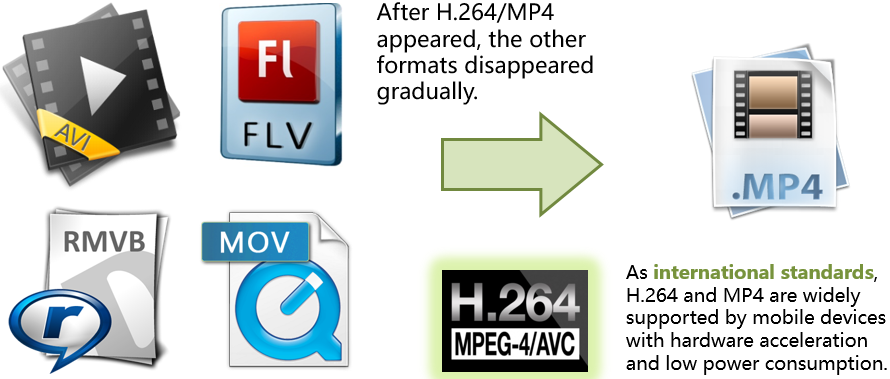
\includegraphics[width=0.80\textwidth]{fig/decisions/video-formats.png} 
	\caption{Changes of prevalent video formats.}\label{fig:video-formats}
\end{figure}

Just as media file extensions have undergone change, computing paradigms have as well. 
Parallel Computing was primary designed to speed up vision and graphics rendering via PC's CPUs and/or GPUs. It required low-level programming with OpenMP, Cilk, TBB, CUDA, OpenCL or other low-level concurrent/parallel libraries. This was then replaced with Distributed Computing. Network and storage capabilities were integrated, while some required hand-written networking or file system operation code. In addition, resource allocation and task scheduling should also be handled by programmers. Today, Cloud Computing has encapsulated the above two, and it relies on another international standard --- the representational state transfer (RESTful) architectural style used for web development. Cloud providers rely on REST so as to improve network management, simplify updates and facilitate safe third party development, as they only expose RESTful APIs to the users or developers at the application layer. 
\begin{figure}[ht]
	\centering
	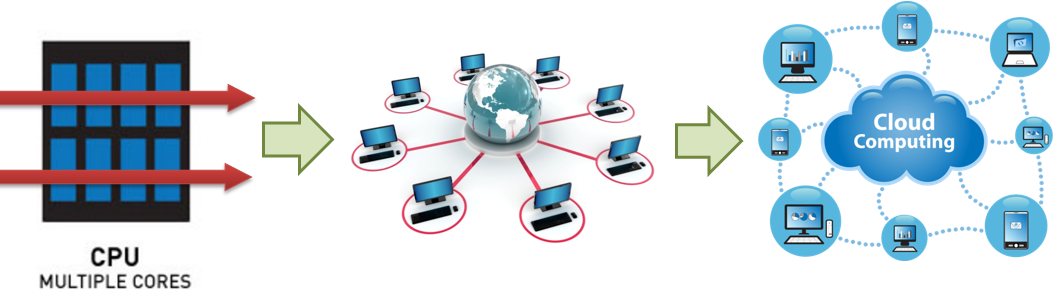
\includegraphics[width=0.80\textwidth]{fig/decisions/parallel-to-cloud.png} 
	\caption{Changes of computing paradigms.}\label{fig:parallel-to-cloud}
\end{figure}

The Cloud RESTful APIs are mostly represented in JSON format. Figure~\ref{lt:googlemaps-api} outlines a JSON response result of Google BigQuery's \texttt{getQueryResults} API. 
\lstinputlisting[caption={JSON Result of a Google BigQuery API.},label={lt:googlemaps-api}]{code/bigquery.json}

One may argue that JSON versus XML is an exception, as XML is an ISO standard but it is used less and less than JSON in many scenarios, such as cloud APIs. However, if you view JSON from another angle, it is a part of JavaScript, one of the ISO-standardised programming languages \cite{ecmascriptiso} \footnote{The current four ISO-standardised programming languages that are still popular are C, C++, Ada, and JavaScript. However, Ada is used only in military applications.}. Besides, JavaScript is now the main language manipulating the Web. 

Going back to the Web, before HTTP and HTML, Gopher was one protocol that facilitated distributing, publishing, searching, and retrieving documents over the Internet. Unfortunately, when the Web became standardised, Gopher almost disappeared from popular applications. 

Before WebRTC, there was another dominant technology that enabled browsers with video/audio decoding, and even P2P capabilities. It was Adobe's Flash plug-in. Flash technologies are 100\% proprietary, as argued in Steve Jobs' letter on Adobe Flash \cite{thoughts-on-flash}, while HTML5 is not. Today, almost all web browsers are moving away from Flash \cite{ff-away-flash}, and even Adobe no longer supports Flash. This transformation will also create lots of new business opportunities. 

Therefore, taking a long-term view, only open and standardised technologies will survive in the future. 

Accordingly, Pear has chosen to embrace several new and upcoming protocols that have just become or will soon become international standards:
\begin{itemize}
	\item Pear mainly uses WebRTC for end-to-end data communication. 
	\item Pear works with DASH for media content representations. 
	\item Pear mainly adopts WebSocket for client-to-server signalling. 
	\item Pear represents its service APIs mainly in JSON, as well as in XML in some places. 
	\item Pear's Fog components are implemented in C, which makes them portable across all types of devices; Pear's initial SDK will be provided in JavaScript, which is the most web-friendly language. 
\end{itemize}

\section{From Cloud to Fog}
\subsection{Problems of the Cloud and Advantages with the Fog}
Here is an incomplete list of current problems of the pure Cloud model: 
\begin{itemize}
	\item Long latency\\
	The communication latency is positively correlated with the physical distance and the number of hops (paths between routers) between the client and the Cloud. More and more financial and industrial applications require millisecond-level latencies, which can hardly be satisfied with pure-Cloud models.   
	\item Wasting power, computation, and bandwidth resources.\\
	In pure-cloud systems, each client has to communicate with the Cloud upon every state-change or data-generation, let alone deal with the pervasive heartbeat messages. Just think about whether it is necessary for data to circle round ({\em i.e.} get transmitted data thousands of km away, get processed, and then delivered back) all the time? Moreover, if there are billions of clients, what kind of pressure will be brought to the backbone networks?  What is worse, clouds consume much more electricity and resources than they truly need. Take China as an example: ``Cloud'' data centres in China consumed 100 billion kWh of electricity in 2014, but only 6\%--12\% was used for processing tasks, and the rest was wasted when servers were idle. 
	\item Still expensive\\
	Most service providers ({\em e.g.} CPs) have to pay a considerable amount of fees for the IDC resources, especially in bandwidth. For some large CPs ({\em e.g.} Tencent), bandwidth cost constitutes over 50\% of the total operational cost. Moreover, the cost of storing historically accumulated data cannot be neglected when the data volume is large, although the cloud storage cost had fallen to less than RMB~0.1 per GB per month as of 2012. 
	\item Single point of failure risks\\
	Remember that clouds have control or ``master'' nodes. Because of routeing and load-balancing needs, data access points are essentially centralised. Today, there is a nefarious underground industry, from which individuals and institutions can easily buy CC, DDoS or NTP amplification attacks, DNS hijacking or poisoning, and even customised intrusion services to harm their rivals or competitors. If one control node is under attack, the service may be unavailable or unreachable. Beyond these, as Internet giants monopolise users' data, information islands can easily be formed due to the lack of a sharing mechanism. One may still remember the cancellation of Google Wave, Google Reader and Google Code, the capacity reduction of Microsoft OneDrive, and the change of allowed synchronised clients of Evernote. If a monopolising giant just changes a single service term or policy, how many data disasters will there be?   
	\item Security and privacy issues\\
	The essentially centralised storage (as well as control or access points) of the Cloud increases the risk of data leakage. Recall \emph{iCloud Nude Leaks} in the US, as well as database ``drag'' incidents of hotel chains, travel agencies, and web forums in China: users essentially have no control over their data stored in clouds, because it is centralised and far away. 
	\item Not being scalable in the ongoing explosion\\
	Suppose a video sharing startup wants to expand to the size of YouTube; will it have enough power resources to transcode all the content in real-time? Alternatively, imagine a gene analytics company wanting to scale up its business to perform DNA sequencing or gene analysis; will it have enough computation power to undertake this task? In the future IoT, a pure Cloud model will definitely not be enough for handling the massive number of constantly-online smart devices that is increasing by orders of magnitude. 
\end{itemize}

Given the above problems of the Cloud, the Fog has definite advantages: 
\begin{itemize}
	\item Its ability to offload the pressure of the Cloud\\
	Fog can undertake simple tasks that eat up a great portion of the Cloud resources.
	\item Physical proximity to end-users\\
	Fog nodes are as near as 0-hop to users, so the Fog can achieve higher performance \& lower delay in most scenarios. Kevin Kelly even predicted that by 2020, over  2/3 of data will be processed locally (within 1km from where it is generated), instead of being uploaded to the ``Cloud''\footnote{\url{http://www.cyzone.cn/a/20141027/264795.html}}. In addition, fog nodes are near users' sensors or computing devices, which are placed in their living environments and generally not accessible directly from remote clouds. 
	\item Low cost\\
	How many Wi-Fi routers are online 7/24? How many unused USB drives do you have? With some \textbf{rebate} incentives, fog has the potential to utilise users' idle resources in a crowdsourcing way, create a new sharing economy in computing and thus lower everyone's costs.  
	\item Eco-friendly characteristics\\
	Most computer programs are either data parallelisable or task parallelisable. In fact, we can achieve linear speedups in most parallelisation work. Obviously, low-power fog nodes are more eco-friendly in processing these tasks (refer to the Section~\ref{sec-dg-vs-dc}).
	\item Huge amount of resources\\
	With a strong and sustainable sharing business model with multiplexing, all Internet users, AP device vendors, operators and service providers can participate in the Fog. 
\end{itemize}

\subsection{Where Fog Works}
\subsubsection{Hardware Resources Analysis of the Fog}\label{sec-hardware-res-analysis}
We now perform an analysis of the different hardware resources in the Fog (Table~\ref{tb:analysis-fog-resources}). 
\begin{table}[ht]
	\small
	\centering
	\caption{Analysis over different types of fog hardware resources.}\label{tb:analysis-fog-resources}
	\begin{tabular}{p{0.16\linewidth}p{0.79\linewidth}}
		\toprule
		Resource Type & Suitable For \\ 
		\midrule
		CPU \& GPU  & Logical \& numerical processing, computing, analytics, rendering, coding, and (deep) learning\\
		RAM            & Data relay, live streaming, VoIP, video conferencing, broadcasting, dynamic accelerations\\
		Storage\tablefootnote{May only be available in some smart APs.}      & VoD, backup, distributed cache \& database, blockchains\\
		IP Address     & Communication, signaling, certain applications requiring a multi-source effect\\
		$\cdots$    & $\cdots$ \\
		\bottomrule 
	\end{tabular}
\end{table}

\begin{table}[htb]
	\small
	\centering
	\caption{First Batch of Fog Applications.}\label{tb:proposed-fog-app}
	\begin{tabular}{llc}
		\toprule
		Applications & Mainly Uses & Estimated Difficulty\\ 
		\midrule
		Media Coding & CPU and GPU cycles & $\star \star \star$ \\
		E-mail Push\tablefootnote{Proposed by Francis Kowk, the CEO of RADICA Systems} & Node IPs/IDs, CPU cycles & $\star \star$ \\
		VPN        & Bi-directional bandwidth & $\star \star \star$ \\
		CDN        & Up-link bandwidth, storage(in VoD)  & $\star \star \star \star \star$ \\
		IoT     & Proximity, reachability, computational power  & $\star \star \star \star$ \\
		Distributed AI & Computational power, storage, network & $\star \star \star \star \star$ \\
		$\cdots$     & $\cdots$  & $\cdots$ \\
		\bottomrule  
	\end{tabular}
\end{table}

\subsubsection{Proposed Applications}
We can abstract a generalised model of fog applications, as depicted in Figure~\ref{fig:fog-generalised-model}. 

\begin{figure}[ht]
	\centering
	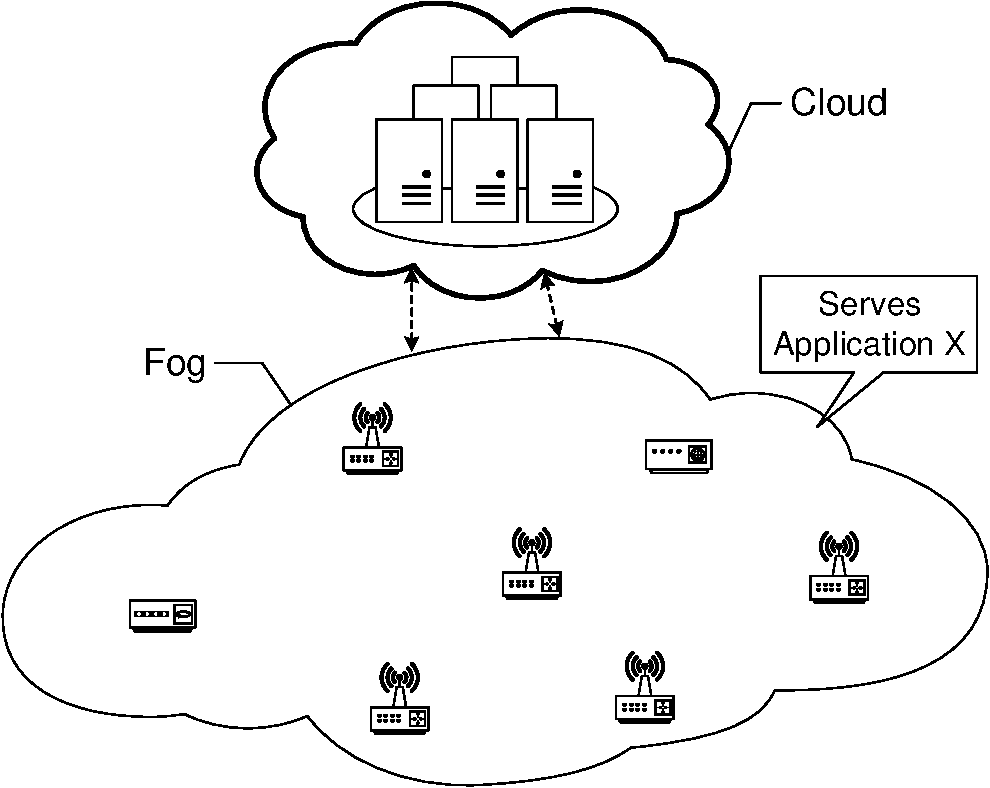
\includegraphics[width=0.75\textwidth]{fig/fog-models/model.pdf}
	\caption{A generalised fog model.}\label{fig:fog-generalised-model}
\end{figure}

We are working on several joint projects that can be launched first, as shown in Table~\ref{tb:proposed-fog-app}. With a \textbf{rebate} scheme, the collaboration will benefit \textbf{all} parties.  

\section{A Stable Hardware Carrier} \label{sec-stable-carrier}% Do hardware!!!
To get a revenue stream to start to flow as quickly as possible, we have to attract contractual or subscribed users. To attract and retain business users, we have to provide a stable, cost-saving and sufficient service. To provide the service, we have to find a sufficient number of suitable hardware carriers powered by Pear's fog programs. Figure~\ref{fig:issue-tree-fog-nodes} shows an issue-tree-like analysis of the hardware carrier solutions. 
\begin{figure}[ht]
	\centering
	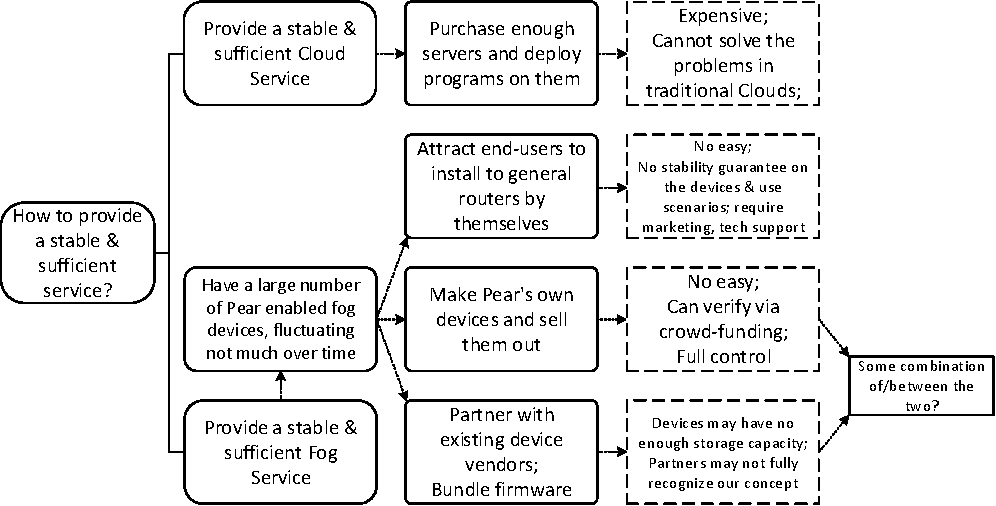
\includegraphics[width=1.0\textwidth]{fig/decisions/issue-tree-fog-nodes.pdf}
	\caption{Issue-tree-like analysis of the hardware carrier solutions.}\label{fig:issue-tree-fog-nodes}
\end{figure}

Individual fog peers can be slow, forbidden, blocked, busy, over-loaded, unavailable, or unreachable. However, to provide fog services, the network size or the system capacity cannot fluctuate too often or too much. Therefore, we had better find stable hardware carriers to run our fog programs on. 
As analysed in Section~\ref{sec-dev-hardware}, we have considered designing an all-in-one hardware device. Whatever form the hardware takes, it should have some AP capabilities, so the devices can serve as home/business Wi-Fi routers and gateways. Below are some of their attributes, online patterns, and advantages in their use scenarios: 
\begin{itemize}
	\item Stable\\
	In fact, most AP devices in the real-world are online 24/7, so our devices should be too.
	\item Relieving us from some NAT traversal problems\\
	Most APs themselves are NAT devices with dedicated IP addresses. With simple port-forwarding tricks, a considerable number of the devices can work as fog servers that can be accessed from outside. 
	\item Transparent and tolerable resource-scheduling plans\\
	Different from the traditional P2P applications 10 years ago, which would ``steal'' the resources on PCs to serve others, scheduling the resources on AP devices to provide fog services has no influence over the users' Internet services since they are not devices the users are \emph{using} directly. In addition, we have monetised incentives for initial acceptance as well as ongoing tolerance of occasional bandwidth reduction (during some peak hours). 
	\item Hardware compatibility and utility\\
	The APs should be very versatile, as discussed in Section~\ref{sec-hardware-res-analysis}. 
\end{itemize}

To find a suitable hardware carrier, another thing we must do is to estimate the processing power in terms of ``performance per dollar''. 
After analysing different types of devices, we found that the current TV-boxes can meet our three main requirements:
\begin{itemize}
	\item Meet our basic needs for running most fog components
	\item Have a lower cost than most other types of devices
	\item Have low energy consumption --- less than 15W Thermal Design Power (TDP)
\end{itemize}

It is hard to measure the performance in a single index or metric, but from the models in Table~\ref{tb:device-comparision}, we can easily see that a TV box is the most suitable platform to run Pear's fog programs, in terms of performance per unit of cost.  

%\doublerulesep 0.1pt
\begin{table}[htb]
	\small
	\centering
	\caption{Performance-Price Comparisons of Different Types of Devices}\label{tb:device-comparision}
	\begin{tabular}{p{0.13\linewidth}p{0.25\linewidth}p{0.25\linewidth}l}
		\toprule
		Device Type & Smart Phone & TV Box & Wi-Fi Router \\
		\midrule   % \parbox[t]{\linewidth}{ARM A7 2.2Ghz $\times$ 4 + \\ARM A17 1.7GHz $\times$ 4}
		CPU & \parbox[t]{8cm}{ARM A7 $2.2$\,Ghz $\times$ $4$ + \\ARM A17 $1.7$\,GHz $\times$ $4$} & ARM A7 $1.3$\,GHz $\times$ $4$ & MIPS 24KEc $580$\,MHz $\times$ $2$\\
		GPU & PowerVR G6200 & Mali-400MP2 & N/A\\
		RAM & $2$\,GB DDR3 & $1$\,GB DDR3 & $128$\,MB DDR2\\
		ROM & N/A & $128$\,MB NAND Flash& $64$\,MB Nor Flash\\
		Storage & $32$\,GB eMMC & $8$\,GB eMMC & N/A\\
		Cost & CNY~$500$ & CNY~$80$  & CNY~$100$\\
		\bottomrule
	\end{tabular}
\end{table}

From Table~\ref{tb:device-comparision}, we can see that the Pear smart router's ``all-in-one'' feature and the ``ARM'' facts and trends make it an easy choice for our hardware carrier. Regarding the Operating System, we will use embedded Linux first, and then later port all components to native programs on Android. Here is our rationale:
\begin{enumerate}
	\item Embedded Linux distributions, like OpenWrt, are widely used in smart routers.\\
	So to utilise the existing components, we had better build on systems like OpenWrt.
	\item The Android OS has the strongest ecosystem currently.\\
	It works not only on smart phones, but also on TV-boxes, tablets, projectors, PCs, watches, and it should work on routers in the near future. Its community is even stronger than Windows. 
	\item The technology that wins the developers wins the world.\\
	This has been proven many times. 
\end{enumerate}

Finally, we will partner with existing hardware vendors, and at the same time, cooperating with them to make our own ``exemplary'' fog devices. Table~\ref{tb:pear-device-spec} shows proposed specifications of Pear's fog node device. 
\begin{table}[htb]
	\small
	\centering
	\caption{Proposed specifications of Pear fog device (smart router).}\label{tb:pear-device-spec}
	\begin{tabular}{lc}
		\toprule
		Component & Specification\\
		\midrule 
		OS  & Linux, or Android with OpenWrt port\\
		CPU & Intel Atom or Core M or ARM Cortex, Quad Core\\
		GPU & Intel HD Graphics or ARM Mali\\
		RAM & 1-4GB DDR3\\
		ROM & 4GB NAND Flash\\
		Storage & 32-128GB eMMC/HFS onboard, SSD/HDD extendible\\
		Slots/Connectors & USB3.0 or Type C, SD/MMC\\
		Networking & 100/1000Mbps Ethernet, 802.11ac Wireless\\
		Shape & Compute Stick, or TV-Box like\\
		Functionalities & Mini-server, NAS, Wi-Fi router, TV-Box, USB Drive\\
		\bottomrule
	\end{tabular}
\end{table}

\section{Fog for Content Delivery}
Among all the potential revenue streams, fog content delivery is paramount. Below we justify its superiority over traditional content delivery over the Cloud, and then we list some key objectives in such content delivery systems. 
\subsection{In Content Delivery, Where Fog Works Better}  % Time in-sensitive!!!

For retrieving an image, a web page, a JavaScript, Flash, or CSS file, which is likely to be a few dozens of KBs in size, fog can hardly beat Cloud. Typically this kind of job can be done within a few hundreds of milliseconds, even taking the RTT into account. By contrast, in a typical fog system which is organised in a structural P2P fashion, where peers and resources are indexed by DHTs. Each query is expected to be routed through a few $\log(n)$ hops (where $n$ is the network size), so roughly throwing these jobs to the Fog will induce a large delay. 

Even in traditional CDNs, handling small-sized data is usually done in a reverse-proxying fashion, as: 
\begin{enumerate}
	\item there might also be routeing delay in querying the cloud storage system; 
	\item redirection mechanisms such as HTTP 302 incur a considerable delay that is much higher than the transmission/processing time.  
\end{enumerate}
Figure~\ref{fig:cdn-req} depicts different request-response models in CDNs. 

\begin{figure}[ht]
	\centering
	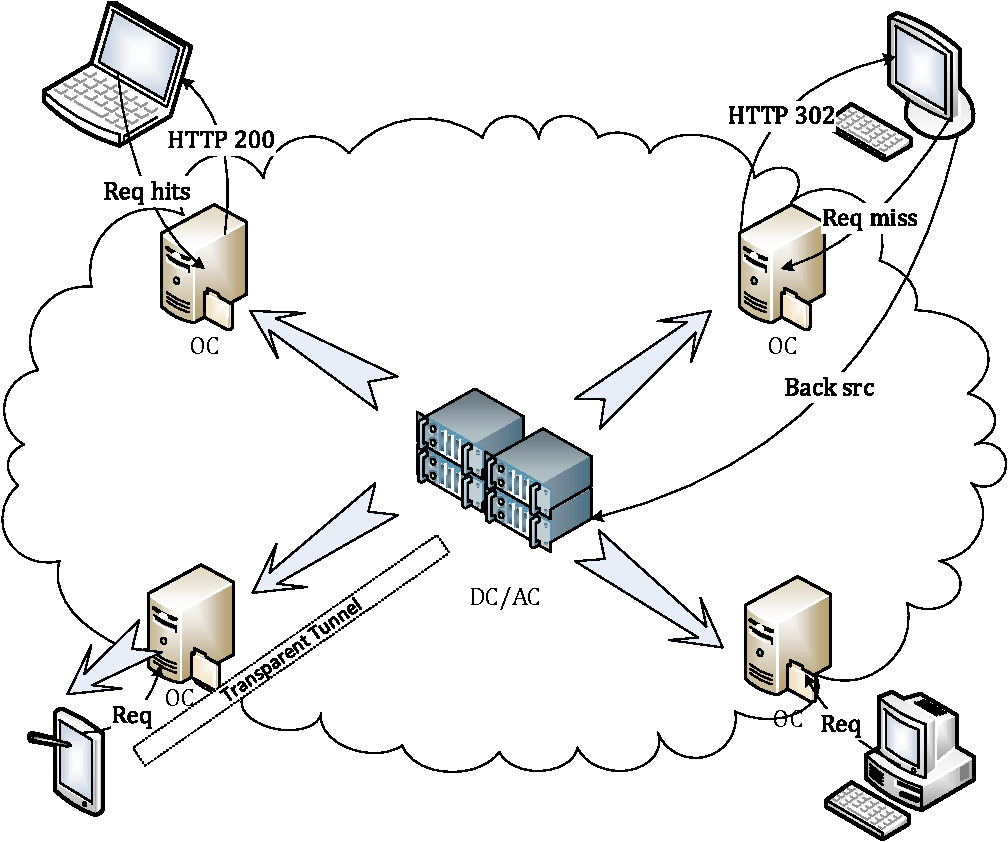
\includegraphics[width=0.72\textwidth]{fig/decisions/CDN_req.pdf}
	\caption{Request-Response models in CDNs.}\label{fig:cdn-req}
\end{figure}

We do not even need to mention fog, which is obviously not suitable for small sized static content. Instead, we further analyse the use of fog in four different content service scenarios:
\begin{description}
	\item[VoD.] VoD is mostly latency-tolerable; fog takes on the relatively hot portion of all content. Fog helps achieve two main benefits: 
	\begin{itemize}
		\item High total bandwidth along the edge with higher distribution density\\
		Even if the per-connection rate is limited, we can aggregate the bandwidth with the help of multi-connection effects. 
		\item Low bandwidth fees at the edge.\\
	\end{itemize}
	\item[Web Content.] This application is time-sensitive in content accessibility, and the data volume is huge. Fog only helps with the large-sized files. In terms of popularity, the hottest portion is already cached in traditional CDN edge regions and the coldest portion should be placed in data centres. Fog mainly helps the medium popularity content objects that are not popular enough to be cached on Cloud CDN edges. Fog helps achieve:
	\begin{itemize}
		\item Relatively low latency if with a considerable replication density
		\item Lower bandwidth cost for content providers
	\end{itemize}
	\item[Live Streaming.] For interactive scenarios, fog is not suitable, because the application is too time-sensitive. Fog can well undertake 10-second to 2-minute delay channels, for example, live broadcasting and live event streaming with low or no user-interaction. 
	\item[Historical Internet Archives.] These have huge amounts of files. When equipped with large storage capacities, fog nodes can also help to quickly replicate the cold portion, providing CPs with a multi-path delivery channel or failover solution. 
\end{description}

\subsection{Key Objectives for Fog Content Delivery}
In this section, we list the key objectives of Pear's fog platform. This can also be deemed as an extension with architectural solution answers to the ``pillars'' part of the OpenFog white paper \cite{openfog}. 
%Connectivity, Security, Interoperability, Transparency, Reliability, Availability, Serviceability, Scalability, Autonomy, Programmability, Proximity, Efficiency, Resiliency(Elasticity), Performance, Agility, Functionality, Utility, Hierarchy ...  Robustness  Profitability!!! (commerciality)    change to descriptions:
\subsubsection{Connectivity, Reliability, Availability, Serviceability, Durability}
As most user-end network devices are behind NATs and/or firewalls, and IPv6 is still not widely used, NAT traversal is critical in fog systems. 
Although Pear's fog devices are also Wi-Fi APs with NAT capabilities, these devices may work behind users' or ISPs' NATs. 
WebRTC has built-in STUN and ICE components to traverse cone-type NATs. However, a considerable portion ($\approx$ 30\%) of NATs are symmetric.  

Ford {\em et al.}~\cite{Ford:2005:PCA:1247360.1247373} generalised the procedures of NAT traversal. To traverse symmetric NATs with random port assignment ($\approx$ 0.5\% of total routers), Tsai~\cite{sqt2008} proposed an brute-force ``occupying'' method, but it induced too much overhead. Wei~\cite{wei2008new} and Klinec~\cite{Klinec:2014:TSN:2659651.2659698} proposed methods by port prediction. 

We build a hybrid [UPnP] + [PCP] (or [NAT-PMP]) + [ICE] solution to increase the connectivity at fog nodes. If a port mapping by UPnP or PCP can be successfully set up, then our fog nodes can serve as TCP and HTTP servers; otherwise we resort to STUN in ICE to establish a P2P connection on top of UDP. In our STUN implementation, we apply a machine learning-based mechanism to predict the range the next assigning port is likely to fall into. 

We also use the parallel mechanisms in Trickle ICE to reduce the communication set-up delay. 

Hence, our fog program on end-users' ``0-hop'' devices can be seen as a  super Web server that supports both HTTP and WebRTC as well as a P2P node. The architecture of Pear's fog node engine is roughly depicted in Figure~\ref{fig:pear-fog-node-engine}. 

\begin{figure}[ht]
	\centering
	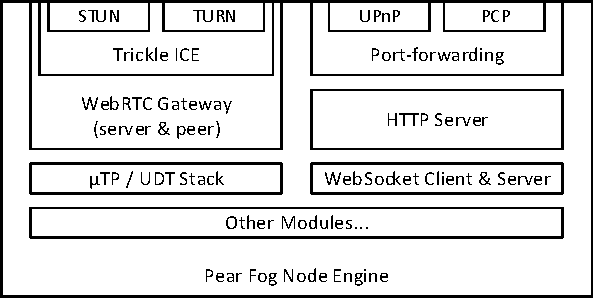
\includegraphics[width=0.75\textwidth]{fig/decisions/pear-fog-node-engine.pdf} 
	\caption{Architecture of Pear's fog node engine.}\label{fig:pear-fog-node-engine}
\end{figure}

The system needs to survive and not fluctuate to some degree. Therefore, durability is a clear success factor. We mainly use monetary incentives to encourage end-users to power and run the devices in a stable and durable fashion. 

\subsubsection{Proximity, Scalability, Autonomy}
Both the Fog and the Cloud provide computation, storage, bandwidth, and application resources. Perhaps the most salient difference between the two is the Fog's proximity to users, the environment, and the underlying accessing nodes. The Fog is more localised, while the Cloud is more generalised. 

In content delivery, to achieve high throughput and to confine traffic within ISPs, years ago, the Global Network Positioning (GNP) method was introduced. Its key idea is to approximately represent the complex structure of the Internet by a simple geometric space ({\em e.g.} an N-dimensional Euclidean space). In this representation, each host in the Internet is characterized by its position in the geometric space with a set of geometric coordinates. Usually, a number of stable servers are used as landmarks. 

However, Choffnes~{\em et al.}~\cite{net-pos-edge} revealed that the Internet positioning from the edge at scale exhibits noticeably worse performance than previously reported in studies conducted on research testbeds. A few hundred of landmarks might be needed to capture most of the variance. 

We devised an online node clustering method in which peers \texttt{ping} each other and form groups in an Expectation-maximisation (E-M) like way. With the help of Radix-tree and GeoHashing, our system allows fast $k$NN and range queries over the whole Internet topology. 
In the near future, we plan to implement this component into ALTO and DHT protocols. 

Beyond gossip protocols like SCAMP \cite{SCAMP}, we will support hierarchical peer regions/groups.  

\subsubsection{Security}
Security is a big issue across all layers. Security in Pear's fog can be categorised into two aspects:
\begin{enumerate}
	\item Security for CPs' content and control;
	\item Security for end-users' devices, data and privacy. 
\end{enumerate} 

Currently, we do not have enough human resources to ensure a 100\% secure system, but building a TLS layer with bi-directional host verification can ensure security for most of the scenarios in the above aspects. Figure~\ref{fig:TLS-hypo} is a Hypothesis-Tree-like analysis of why to construct this TLS layer at an early stage.  

\begin{figure}[htbp]
	\centering
	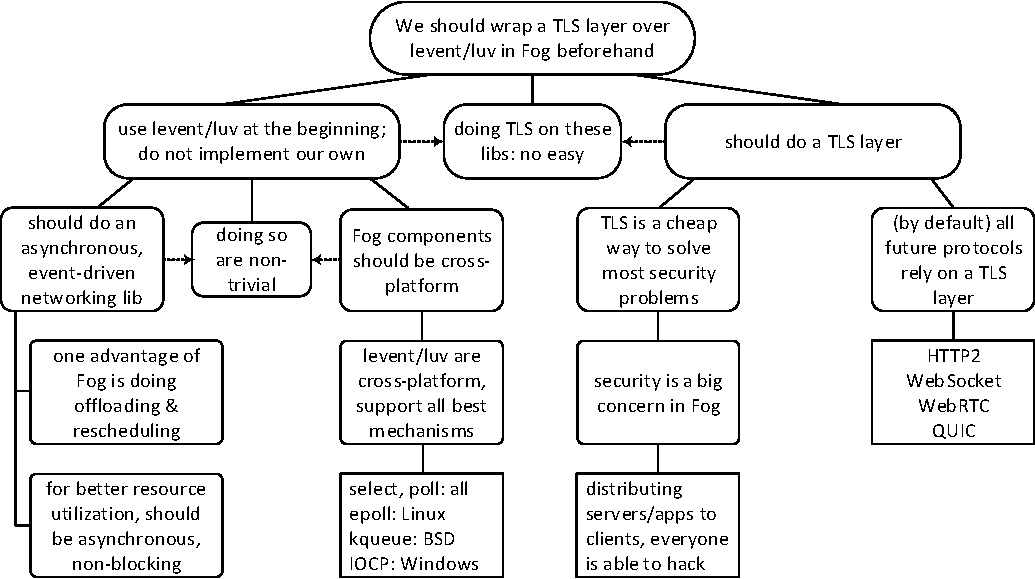
\includegraphics[width=1.00\textwidth]{fig/decisions/tls-hypothesis.pdf}
	\caption{Hypothesis-Tree-like Analysis on the TLS issue}\label{fig:TLS-hypo}
\end{figure}

To ensure data integrity and avoid data being replaced by illegal content, Pear will implement its own Self-verifying File System (SFS) with \texttt{lfuse}. 

\subsubsection{Interoperability, Transparency, Programmability}
WebRTC endows the system with strong interoperability with the Web world. In addition to it, we provide SDKs for different platforms such as Windows, Android and embedded Linux. 
Our SDKs work nearly transparently. Section~\ref{sec-streaming-protocolic} shows a one-line enabling demo for the web front-end. 
We also provide plug-in development capabilities on top of Pear Fog components. To program with Pear Fog, a developer is just required to override or implement a few call-back functions. 

\subsubsection{Efficiency}
Different from BitTorrent's design logic, Pear's Fog system cares more about efficiency than fairness or equality. 
On top of the shared platform and resources, Pear implements different algorithms for different service scenarios. 

\subsubsection{Resiliency, Elasticity, Agility}
We will soon develop an automatic Operating Support System (OSS) that distributes solid and reliable agents to every fog node, partly as described in the U-2 project in Section~\ref{sec-medium-term-projs}. 

\subsubsection{Commerciality, Profitability}
Last but not least, every service the Fog platform provides shall be business-friendly. Cooperating with CPs, Pear is going to create a digital coin and build sustainable monetary incentives. 
As discussed before, we will try our best to introduce a strong Android eco-system to our platform and make the plug-in development profitable. We will try to win the developers --- from the beginning.

\section{The Economy of Attention and User-centric Innovation}
As the amount of information increases, the most valuable resource becomes attention --- not the information itself. During the past decade, most successful marketing philosophies were built on top of ``the economy of attention''. However, this inherently embeds in an ``informing'' thought and often aims at a deal or a transaction. It lacks warmth and ignores the humanistic solicitude of customers. 

Now there is a shift from ``the economy of attention'' to ``the economy of willingness''. 

The customers not only engage in the design but also create and share value among themselves in the communities. It is user-centric: no informing or persuasion -- just touching users' hearts through deeds and matters of the heart. In an era of a willingness economy, engagement in design and production is more important than obtaining the product. The competitiveness of future enterprises will lie on the ability to turn willingness into demand. 

Before turning willingness into demand, we have to create the willingness, and before creating the willingness, we have to build up a good image. Pear partners will actively participate in technical web forums on OpenWrt, Android, or wireless routers. A considerable number of the members of these communities are likely to be Pear Fog's early adopters, both for software and hardware. 
On the other hand, they can also serve as volunteers to help improve Pear's products. 

\section{A Single-point Breakthrough}
For a small start-up, it is not wise to do something which is obviously occupying a giant's main road before it. Instead, most successful start-ups have grown big because they grabbed a narrow trail that had the potential to lead to a broad land where they could dominate. At first, their trails then looked so trivial and non-profitable that the giants saw no value in paying attention, let alone putting resources into them. 

We minimise our potential projects to a single thing: iWebRTC, a smart fog gateway that
\begin{itemize}
	\item supports all Web-friendly protocols such as HTTP, WebRTC, and WebSocket;
	\item supports all P2P-friendly techniques such as uTP, UPnP, PCP (or NAT-PMP), STUN, Trickle ICE, DHT, GOSSIP and ALTO; 
	\item unites the Fog, the Cloud, and the Web. 
\end{itemize} 

It is an all-purpose project that connects: 
\begin{itemize}
	\item the router world and the browser world
	\item the communication domain and the computing domain
	\item the circuit switching net and the packet switching net
	\item the very back-end and the very front-end    
\end{itemize} 

Moving forward, this project enables us to perform domain-specific applications, such as healthcare; going backward, this project enables us to do better traffic-related services. 

We will try our best to make a single-point breakthrough on top of it. We expect that in a foreseeable time ({\em i.e.} 2-3 years), Pear's iWebRTC will be to the real-time data/media communication world what Nginx has become to the Web server field. 

Specifically, in the first stage, even for the WebRTC stack, we will avoid jumping too deeply into the media codec part, because this part is still not settled within the standardisation committee, as it is where giants fight with each other (see Figure~\ref{fig:giants-fight}). 

\begin{figure}[htbp]
	\centering
	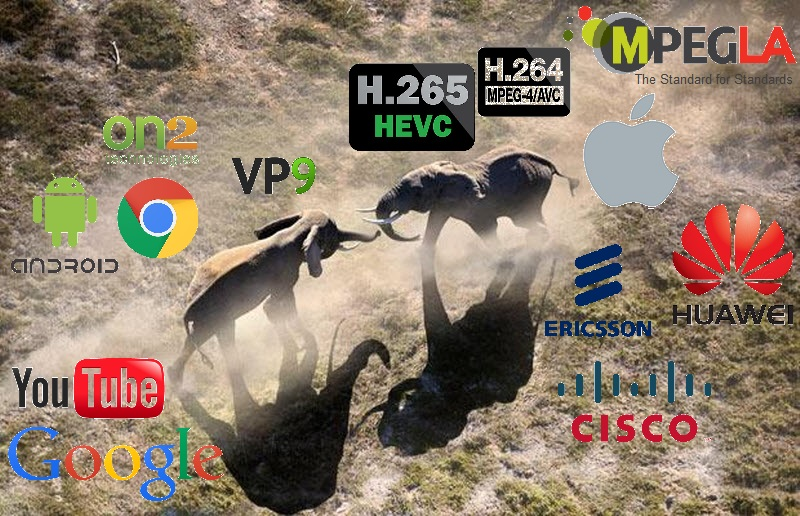
\includegraphics[width=0.86\textwidth]{fig/decisions/giants_fight.jpg} 
	\caption{Video Coding Standards: where giants fight.}\label{fig:giants-fight}
\end{figure}


\section{Three Medium-Term Projects of Pear}\label{sec-medium-term-projs}
\begin{description}
	\item[Manhattan] First of all, we will create a business that utilises the idle bandwidth at the user-end to help with a lot of fog computing scenarios. Our core is the software suite that runs on the devices that process the data requests, plus the ``coordinator'' programs on our servers that optimise the traffic on the whole network. Our architecture and algorithms greatly outperform the traditional ones. It is like an atomic bomb. So we have named this part the ``Manhattan'' project. 
	
	\item[B-29] But even if we successfully make an atomic bomb, we will still be unable to drop it on our enemy -- because it is too far away and we have no long-range carrier. Obviously, we should develop a software launcher beforehand. It must automatically update itself and work in an incremental and peer-to-peer fashion, thus saving bandwidth --- imagine tens of millions of clients: how can we update them all to the latest version in a single day? We need a combination of the advantages of Google's, Microsoft's, and Tencent QQ's updating schemes. We call this one the ``B-29'' project. This project also contains a hardware carrier selection process. 
	
	\item[U-2] After the above two weapons are done, the system will be in operation. To save as much labour-cost as possible, we should also develop a system that monitors and manages the devices anywhere and everywhere. It should also work automatically as much as possible and provide fault-tolerance capabilities. This system is to us in our competition what the U-2 plane was to the US in the cold war. 
	
	\begin{figure}[ht] 
		\centering 
		\subfigure[B-29.] { \label{fig:Manhattan} 
			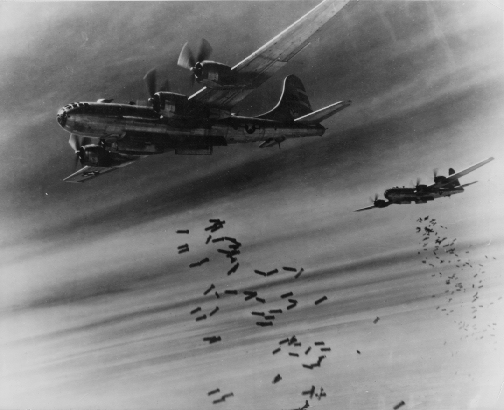
\includegraphics[width=0.33\columnwidth]{fig/decisions/B-29.jpg} 
		} 
		\subfigure[Manhattan.] { \label{fig:B-29} 
			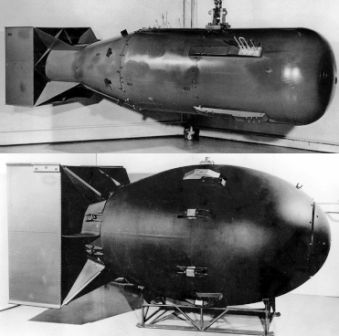
\includegraphics[width=0.27\columnwidth]{fig/decisions/fat-man-little-boy.jpg} 
		} 
		\subfigure[U-2.] { \label{fig:U-2} 
			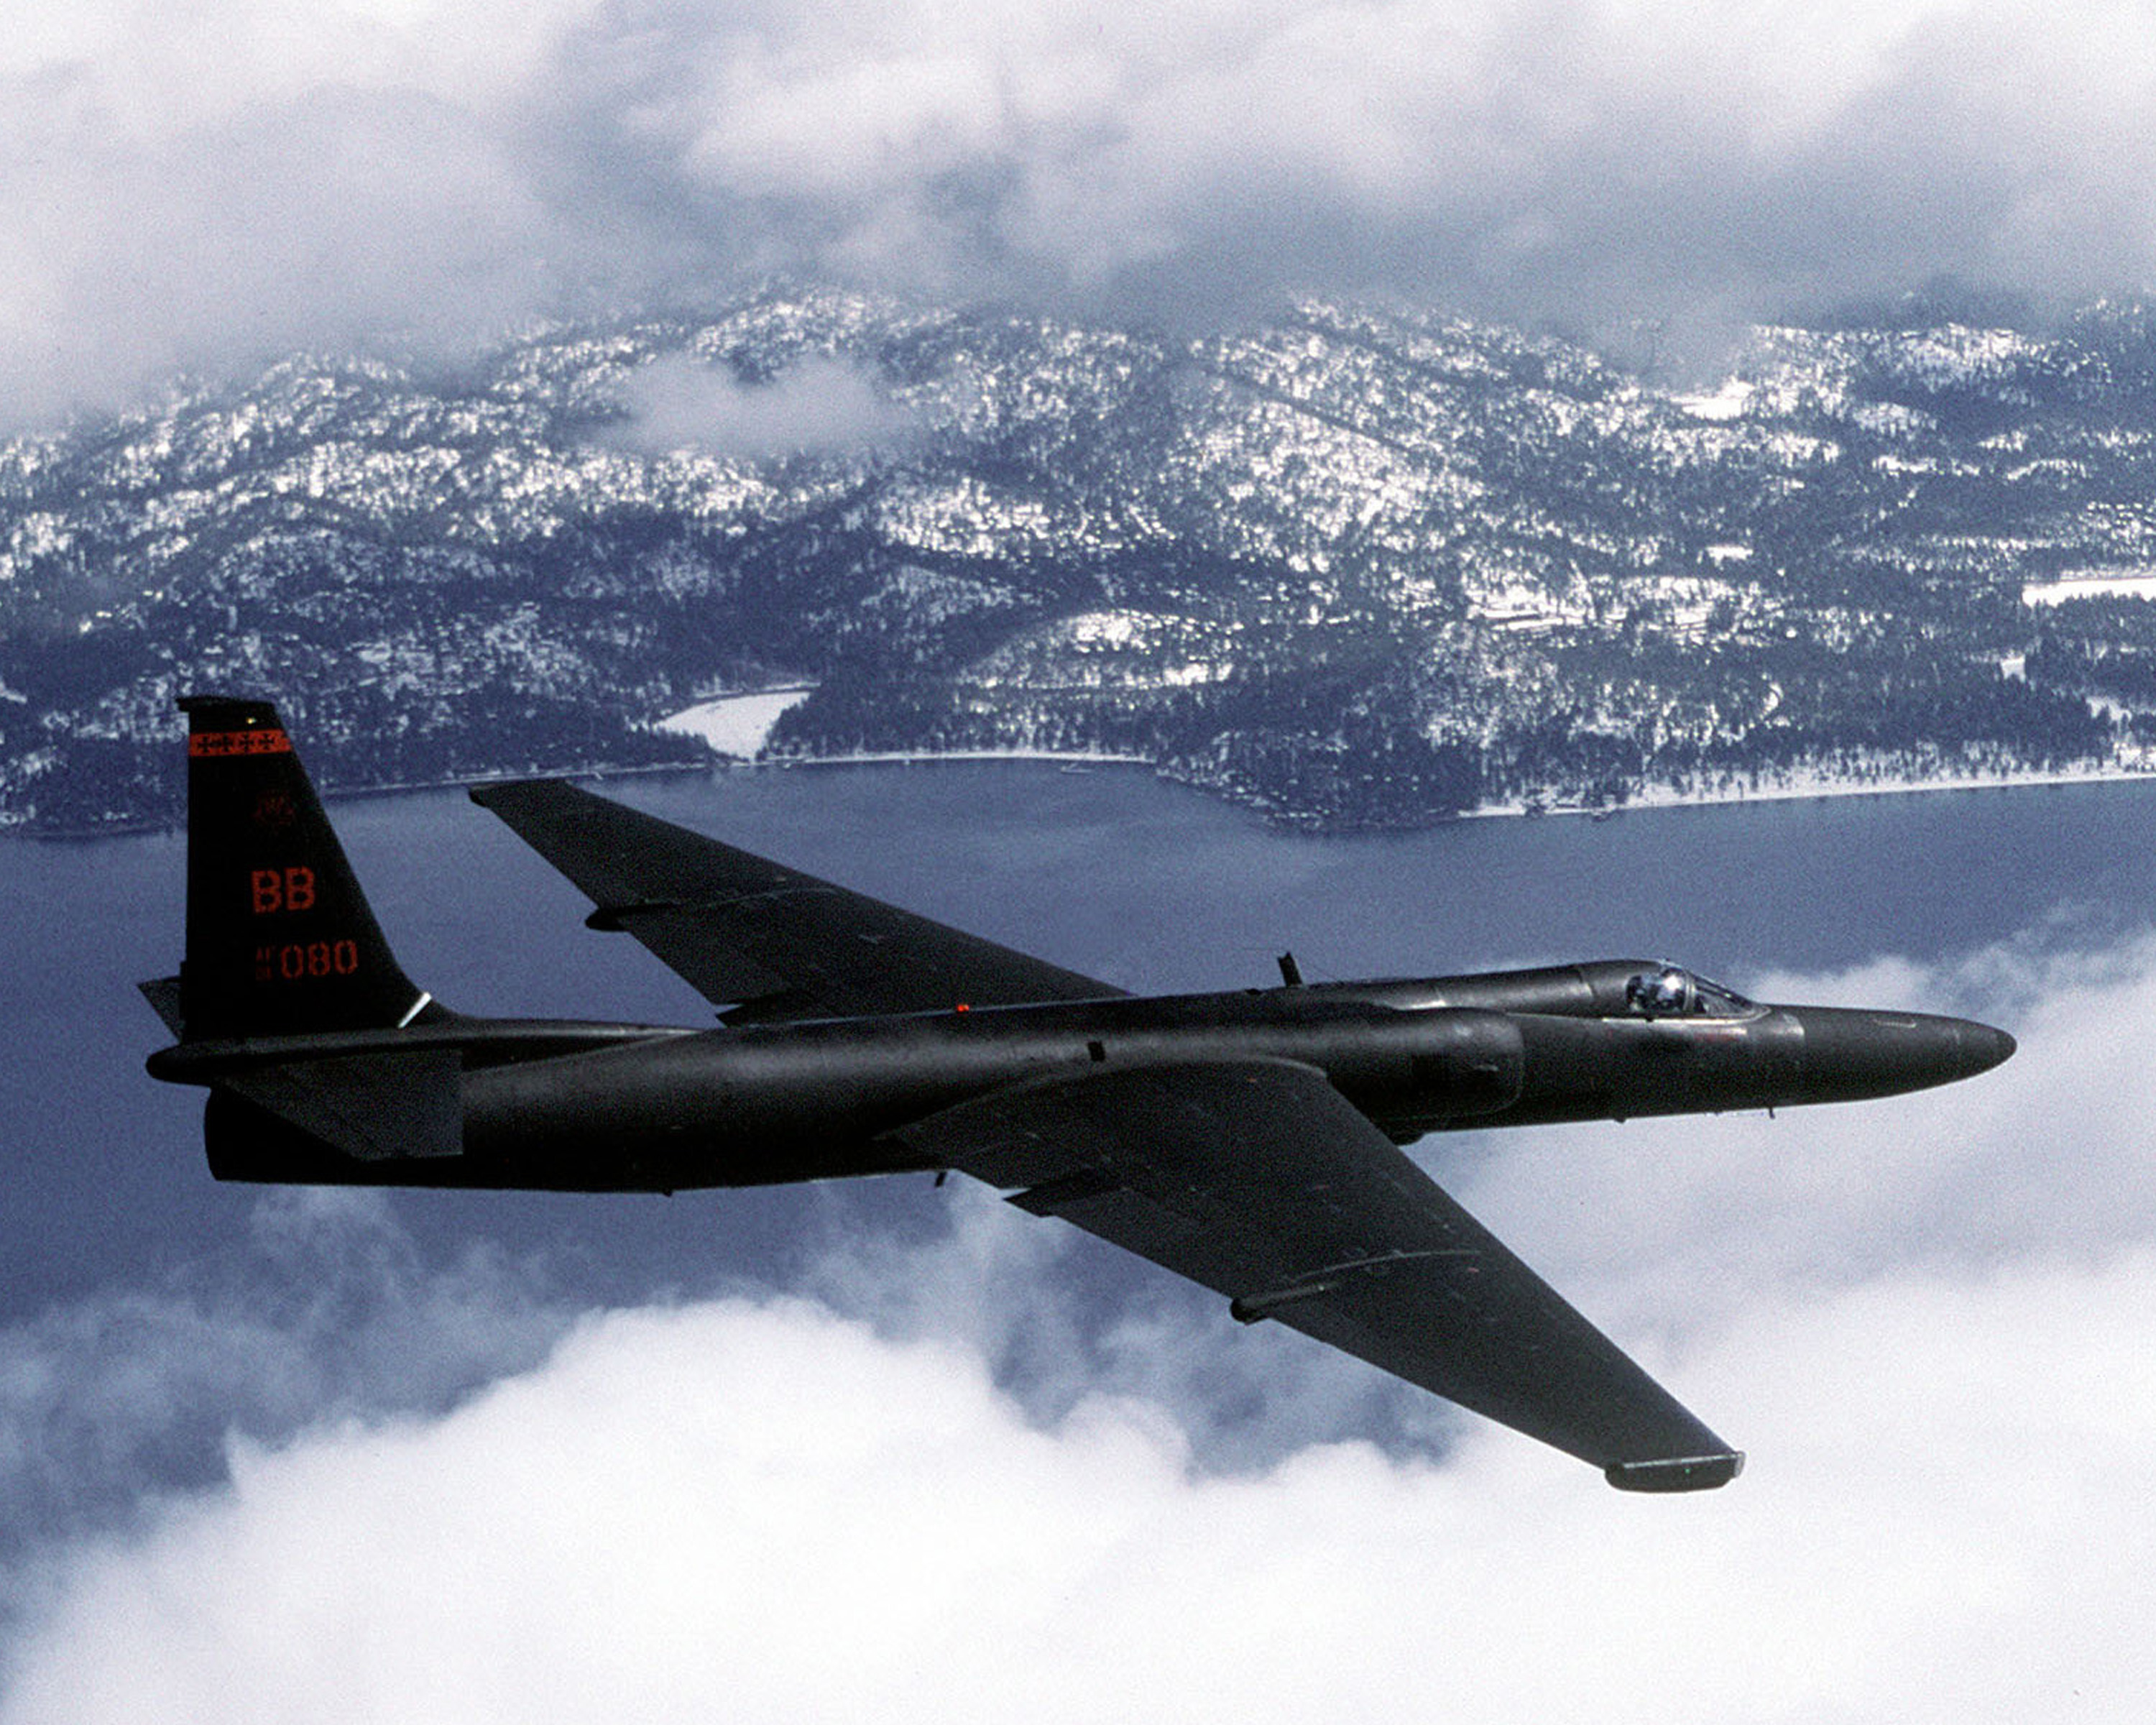
\includegraphics[width=0.33\columnwidth]{fig/decisions/U-2.jpg} 
		} 
		\caption{Three metaphors of the 3 pivotal projects of Pear.} 
		\label{fig:3projs} 
	\end{figure}
\end{description}

\newpage

\chapter{Cooporation Cases}\label{chp-cooporation-cases}
Based on the increasingly mature CDN content sharing platform, the Gehua Chain project team will focus on ``building a trustable, smart, and effective new shared economy'', continuously to exploit the blockchain technology capabilities and enrich the intelligent applications, and build a TSD  (Trust-Security-Development) smart ecology.

\section{Gehua Chain}
Gehua Chain is one of Pear's tailored set of solutions according to the needs of its partners. 

The Gehua Token is a virtual digital proof generated by the Gehua Chain project. Via sharing bandwidth, storage, compute, and other idle resources, Gehua Chain router users can mine tokens issued by the Gehua team. The number of tokens a user receives is according to his/her weight of contribution. 
All the proofs are stored in secure Blockchain. Each of the Gehua Chain router miner users has an account, a password or certificate, and can take effective operations on top of his/her proofs.

\subsection{Use Scenarios of the Gehua Token}
The Gehua Token works as the exchange medium for the TSD smart sharing ecosystem in two ways: 
\begin{enumerate}
	\item It is used by many content providers to purchase TSD services ({\em e.g.} Fog CDN services). As such, we define it as a utility token. 
	\item Miners can use it to exchange for digital contents or other digital services ({\em e.g.} membership fees). Here the Gehua Token is a currency token as it is a medium of value exchange. 
\end{enumerate}
The Gehua token is not an asset token, therefore it does not offer any dividends profits or voting right. While there will be direct or indirect ways to exchange Gehua Token to or from other digital cryptocurrencies or fiat currencies, the main purpose of Gehua Token is to be the utility token within the Gehua Chain ecosystem. 

\subsection{Distribution of the Gehua Token}
The Gehua Token adopts the PoS (Proof of Stake) algorithm, taking the device's hardware (compute and memory) capability, bandwidth capability, storage capability, traffic contribution, and online duration into account. 

In each digital PoS period $t$, $n$ is the total number of valid online nodes, $c$ is the total amount of tokens to be issued, then $c$ is divided into 4 parts: hardware capability, bandwidth capability, storage capability, traffic contribution: 
\begin{equation}
	c = c_h + c_s + c_b + c_d
\end{equation}

We denote their weights as: $w_h = \frac{c_h}{c}, w_s = \frac{c_s}{c}, w_b = \frac{c_b}{c}, w_d = \frac{c_d}{c}$, apparently $w_h + w_s + w_b + w_d = 1$. Here is a sample tuple of values: $w_h = 0.2, w_s = 0.3, w_b = 0.2,  w_d = 0.3$. 

The digital certificate $c(i)$ obtained by node $i$ consists of 4 parts:
\begin{equation}
	c(i) = c_h(i) + c_s(i) + c_b(i) + c_d(i)
\end{equation} 

$c_{*}(i)$ is decided by the ratio of the current total circulation in one category $c_{*}$ multiplied by the power value $p_{*}(i)$ of the node $i$ to the sum of the corresponding capability/contribution values of all nodes: 
\begin{equation}
	c_{*}(i) = c_{*}\times \frac{p_{*}(i)}{\sum\limits_{k=1}^n{p_{*}(k)}}
\end{equation}

For $p_h$, we set the configuration of the first generation router, as the minimum configuration of hardware to mine the Gehua Token, and we assign it the benchmark value of 1. 

For $p_s$, 
\begin{equation}
	p_s = \log{(\frac{s}{S}+1)}
\end{equation}
where $s$ is a measure for the storage space available for mining, and 
\begin{equation}
	s = s_u + \lambda s_a
\end{equation}
where $s_u$ is the space that has already been used for mining, and $s_a$ is the unused space available for mining, $S$ is a measure adjustment parameter and its initial desirable is 250, all in GB. Following the principle of maximum entropy, we set $\lambda = \frac{1}{2}$. 

For $p_b$, we take the minimal of uplink bandwidth $b_u$ and the downlink bandwidth $b_d$, namely $\min(b_u, b_d)$. 

We calculate the Internet data traffic that each node contributes every five minutes and we get a total of 288 values a day. We record it as a vector $\vec{d}$ of length 288. In the region/time zone where the node is located, the value of Internet data traffic of each time slot corresponding to 5 minutes is not the same, and is denoted as vector $\vec{v}$. Then we have: 
\begin{equation}
	p_d = \vec{d} \cdot \vec{v}
\end{equation}

We can set maximum values for $p_h, p_s, p_b, p_d$, no additional mining reward a node can earn if any of its power value exceeds a given one. The weights $w_h, w_s, w_b, w_d$, $S$ and $\lambda$ will also be voted on, updated and publicised through a committee constitutes of three parties: miners, fog service clients, and the Gehua team. 
\specialchapter{Acknowledgements}
%Font "test";  ··test··; ``test"; ``test'': \texttt{texttt}; \textsl{textsl}; \emph{emph}; \textsc{textsc}; \textsf{textsf}; \textit{textit}
The ``crowd-sourced fog'' idea that is explained in this white paper has evolved and been practised for over five years. I rejoice that the number of its direct and indirect contributors has grown so great that the full recognition of all people who have made it possible is regretfully impractical. 

I first thank my advisor, Professor S.-H. Gary Chan, for his years of mentoring and encouragement. I have learned from him how to define, decouple, differentiate, develop and defend problems and ideas. From him, I have gained the habit of being systematic, structural, punctual and precise. I am also very grateful for his recommendation of me to the Technology Leadership and Entrepreneurship (TLE) program. 

Stone Huang at Tencent Cloud, has provided wise counsel throughout the evolution of this work since the very beginning. I am grateful to Zhi Wang and Wen Hu for the inspiring collaboration at the Tsinghua-Tencent Joint Laboratory for Internet Innovation Technology and to Wenwu Zhu for his advice. I thank Les Peng and Isco Wei at the Tencent Social Network Group (SNG) for their technical support. I thank many others at Tencent Technology and Engineering Group (TEG) for their roles in deploying code and providing data, as well as people I worked with at other organisations who were a source of inspiration for this project.  
%All my previous working experiences with respective institutions constituted a source of inspiration for this project. 

I am grateful for the support from the Hong Kong University of Science and Technology (HKUST) in its unwavering commitment to excellence in teaching, learning and research, especially its vision for future entrepreneurship education. Thanks to the School of Engineering, which conducts the TLE program and practises future-oriented educational experiments. Thanks to the School of Business and Management, where I attended some ``secret-weapon'' MBA courses, learned some practical business problem-solving skills and then reversely applied them to help analyse some technological problems. 

I acknowledge my teachers and colleagues who provided such supportive and stimulating environments, especially King Lun Yeung, Margaret Chau, Wendy Yau, Jenny Chan and Louise Yap at the Office of the Dean of Engineering and the TLE program, Qiang Yang of the Department of Computer Science and Engineering, Laurence C Franklin of the Department of Finance and the MBA program, as well as Sam Garg of the Department of Management. 

I am indebted to Mitchell M Tseng for encouraging me to do a real start-up, to Terrence F Yee for helping me sort out some IP issues, and to Claudia J Xu and Brian Sze for helping us receive some government funding through HKUST. 

I especially want to thank Tony Zhang, the co-founder and ex-CTO of Tencent, for pointing out the ``dominant battlefield'' of the Fog, and John Lu of the Tencent Video team, for helping polish the ideas and direct the project to a key problem related to a better ``carrier''. 

I want to express my gratitude to Po Chi Wu, who has given helpful suggestions and allowed our project to be case-studied in a business course. 

I appreciate the lessons learned from many friends, who did start-ups, organised influential competitions, or administrated laboratories. They include Hamza Zia (Parle), Pili Hu (Initium Media), Peter Chung (CSE Office and HackUST), Wen Huang (MTrec Lab. and AnanFlow), Francis Kwok (RADICA Systems) and Michael Huang (Maichuang Networks and ViewCloud). 

I am obliged to Yuqing Lin, Michael Xue and Cindy Liang at Lenovo Capital, for their insightful comments on improving this work. I am grateful for Camden Meek's and Ted Spaeth's help in document editing.  

The collaborators in the Pear Team --- Ian Mei, Yongming Li, Pearl Shu and Evian Ling, who also have my gratitude. Through collaborative work, I am able to understand what kind of people a start-up should look for. I also want to thank Raymond, Michael, Hammad, Gavin, Peipei, Shuya and July, who helped enhance Pear's capabilities and avoid risks in different dimensions. 

I owe thanks to Yolanda Yang, Gordon Yen and Derek Liu for many interesting discussions, and to the anonymous referees for many helpful suggestions.

Last but not least, I thank my parents, for their full support for my projects and the start-up company. I affectionately dedicate this white paper to them. 



\bibliographystyle{IEEEtran}  % 2nd choice: plain
\bibliography{IEEEabrv,ref}
\addcontentsline{toc}{chapter}{References}
\end{document}
